
\documentclass[runningheads]{llncs}

\usepackage{fontspec}
\setmainfont{Times New Roman}
\usepackage{graphicx}
\usepackage{url}
\usepackage{hyperref}
\usepackage{amsmath}
\usepackage{booktabs}
\usepackage{enumitem}

\setlength{\emergencystretch}{2em}

\begin{document}

\title{Nhận diện và phân tích giá xe hơi ở Việt Nam}
\titlerunning{Phân tích dữ liệu ô tô Việt Nam}

\author{Phạm Trọng Nghĩa\inst{1} \and
    Trần Công Vinh\inst{1} \and
    Trần Quang Duy\inst{1}}

\authorrunning{P. T. Nghia et al.}

\institute{Học phần PPR501, FSB-MSA\\
    \email{Giảng viên hướng dẫn: Nguyễn Xuân Sâm}}

\maketitle

\begin{abstract}
    Báo cáo trình bày dự án phân tích dữ liệu ô tô tại Việt Nam
    thông qua ba hướng tiếp cận: Linear Regression để khảo sát và
    ước lượng giá xe, Convolutional Neural Network (CNN) để phân
    loại ảnh xe, và Vision Transformer (ViT) như một hướng tiếp
    cận dự kiến cho bài toán phân loại ảnh. Phần phân tích giá
    sử dụng dữ liệu rao bán xe, chuyển đổi giá từ các đơn vị
    ``Tỷ'' và ``Triệu'' sang triệu đồng, sau đó khảo sát mối
    quan hệ giữa năm sản xuất và giá xe. Ứng dụng Streamlit
    hỗ trợ xem dữ liệu, lựa chọn biến đầu vào và mục tiêu,
    huấn luyện mô hình, trực quan hóa kết quả và thử dự đoán.
    Phần phân loại ảnh sử dụng bộ dữ liệu gồm bảy nhóm xe.
    Notebook hiện có ghi nhận accuracy trên tập test khoảng
    68,76\% và loss khoảng 1,1721 sau 20 epoch. Đối với ViT,
    báo cáo đề xuất quy trình thực nghiệm nhằm khảo sát khả năng
    áp dụng Transformer vào phân loại ảnh xe và tạo cơ sở so
    sánh với CNN. Tuy nhiên, ViT chưa được triển khai trong
    phiên bản hiện tại nên chưa có kết quả thực nghiệm. Báo cáo
    phân tích các giới hạn về tiền xử lý, đánh giá mô hình và
    khả năng tái lập, đồng thời đề xuất các bước hoàn thiện
    thực nghiệm trong tương lai.

    \keywords{Phân tích dữ liệu \and Ô tô \and Linear Regression
        \and CNN \and Vision Transformer \and Machine Learning}
\end{abstract}

\section{Giới thiệu}

Thị trường ô tô có thể được khảo sát thông qua dữ liệu rao
bán và hình ảnh phương tiện. Dữ liệu có cấu trúc cung cấp
thông tin về giá, năm sản xuất, số kilomet đã đi và các
thuộc tính của xe. Trong khi đó, hình ảnh cung cấp thông
tin trực quan có thể được sử dụng để nhận diện nhóm xe.

Dự án ``PPR501 Car Analysis'' tập trung vào hai nhóm bài
toán chính. Nhóm thứ nhất là phân tích và ước lượng giá xe
từ dữ liệu có cấu trúc. Nhóm thứ hai là phân loại hình ảnh
xe bằng các mô hình học sâu. Trong nhóm bài toán thị giác
máy tính, CNN là phương pháp đã được triển khai, còn Vision
Transformer (ViT) được đề xuất như một hướng mở rộng để
nghiên cứu khả năng sử dụng cơ chế self-attention trong
phân loại ảnh xe.

Mục tiêu của dự án là xây dựng các công cụ minh họa có thể
tương tác, giúp người dùng quan sát dữ liệu, thử dự đoán
và tìm hiểu cách áp dụng các phương pháp Machine Learning
vào bài toán ô tô. Dự án đồng thời xem xét các giới hạn của
quy trình huấn luyện và đánh giá để xác định những cải tiến
cần thiết.

Các câu hỏi nghiên cứu được xác định như sau:

\begin{enumerate}[label=\textbf{RQ\arabic*.}]
    \item Linear Regression có thể được sử dụng như một
          baseline để khảo sát mối quan hệ giữa năm sản xuất và
          giá xe như thế nào?
    \item CNN có khả năng phân loại hình ảnh xe thuộc bảy
          nhóm đã xác định ở mức độ nào theo kết quả hiện có?
    \item Vision Transformer có thể được triển khai để giải
          quyết cùng bài toán phân loại ảnh xe, và cần những
          điều kiện thực nghiệm nào để so sánh với CNN?
\end{enumerate}

Trong phạm vi phiên bản hiện tại, hai phương pháp Linear
Regression và CNN đã có phần triển khai. ViT mới ở giai
đoạn đề xuất, do đó câu hỏi RQ3 chưa được trả lời bằng
kết quả thực nghiệm.

\section{Cơ sở lý thuyết và nghiên cứu liên quan}

\subsection{Linear Regression}

Linear Regression là phương pháp hồi quy có giám sát được
sử dụng để mô hình hóa mối quan hệ giữa biến đầu vào và
biến mục tiêu. Với một biến đầu vào, mô hình giả định mối
quan hệ tuyến tính giữa đặc trưng và giá trị cần dự đoán.

Ưu điểm của phương pháp là dễ triển khai, dễ diễn giải và
phù hợp để xây dựng baseline. Tuy nhiên, giá xe chịu ảnh
hưởng của nhiều yếu tố và các mối quan hệ này không nhất
thiết là tuyến tính. Do đó, mô hình sử dụng riêng năm sản
xuất không thể đại diện đầy đủ cho toàn bộ quá trình hình
thành giá xe.

\subsection{Convolutional Neural Network}

CNN là kiến trúc mạng nơ-ron thường được sử dụng trong xử
lý ảnh. Các lớp convolution học đặc trưng không gian từ
ảnh, trong khi pooling giảm kích thước biểu diễn và hỗ trợ
xây dựng đặc trưng ở mức cao hơn. Các lớp fully connected
sử dụng đặc trưng đã trích xuất để dự đoán nhãn.

Trong dự án này, CNN được sử dụng làm mô hình phân loại
ảnh xe đã triển khai. Kết quả của mô hình là cơ sở ban đầu
để đánh giá khả năng nhận diện bảy nhóm xe.

\subsection{Vision Transformer}

Vision Transformer được giới thiệu bởi Dosovitskiy và cộng
sự, áp dụng kiến trúc Transformer cho bài toán phân loại
ảnh. Thay vì chỉ sử dụng các phép tích chập, ViT chia ảnh
thành các patch, chuyển chúng thành vector biểu diễn và
xử lý chuỗi vector thông qua các Transformer Encoder.

Cơ chế self-attention cho phép mô hình học quan hệ giữa
các patch trong ảnh. Tuy nhiên, hiệu quả thực tế phụ thuộc
vào kiến trúc, dữ liệu, trọng số khởi tạo và cấu hình huấn
luyện. ViT không mặc nhiên tốt hơn CNN trong mọi bài toán,
đặc biệt khi dữ liệu huấn luyện có quy mô hạn chế.

Trong phạm vi dự án, ViT được đề xuất để phân loại cùng
bộ dữ liệu ảnh xe với CNN. Việc sử dụng trọng số pretrained
và fine-tuning là một phương án cần khảo sát nhằm giảm
nhu cầu huấn luyện từ đầu.

\section{Dữ liệu và tiền xử lý}

\subsection{Dữ liệu giá xe}

Dự án sử dụng tệp \texttt{car-price.csv} lấy từ Kaggle
\cite{carprice}. Theo thông tin hiện có của dự án, tệp
gồm 15.442 dòng và 17 cột. Các thuộc tính bao gồm giá,
năm sản xuất, số kilomet đã đi, tình trạng, xuất xứ, kiểu
dáng, động cơ và các thông tin khác trong tin đăng. README
của dự án mô tả dữ liệu bao phủ giai đoạn 1990--2023.

Giá xe được lưu dưới dạng văn bản có thể chứa đơn vị
``Tỷ'' và ``Triệu''. Để phục vụ phân tích số, giá được
quy đổi về triệu đồng Việt Nam. Phần giá tính theo tỷ
được nhân với 1.000 rồi cộng với phần giá tính theo triệu.

Quá trình tiền xử lý cần loại bỏ hoặc xử lý những dòng có
giá không hợp lệ, giá trị thiếu và các trường hợp không
thể chuyển đổi sang kiểu dữ liệu số. Các bước này cần được
kiểm tra khi chạy lại để bảo đảm số lượng quan sát sử dụng
trong mô hình là rõ ràng và có thể tái lập.

\subsection{Dữ liệu ảnh xe}

Bộ dữ liệu ảnh được lấy từ nguồn Kaggle
\cite{carimages}. Theo notebook hiện có, dữ liệu gồm
3.352 ảnh train và 813 ảnh test. Các thư mục con tương
ứng với bảy nhãn:

\begin{itemize}
    \item Audi;
    \item Hyundai Creta;
    \item Mahindra Scorpio;
    \item Rolls Royce;
    \item Swift;
    \item Tata Safari;
    \item Toyota Innova.
\end{itemize}

Notebook CNN đọc ảnh ở kích thước $256 \times 256$ và
chuẩn hóa giá trị pixel về khoảng $[0,1]$. Phép xoay ảnh
và lật ngang được sử dụng để tăng cường dữ liệu huấn luyện.

Đối với hướng ViT, kích thước ảnh và phép chuẩn hóa cần
được xác định theo cấu hình cụ thể của mô hình được chọn.
Nếu sử dụng mô hình pretrained, cần áp dụng đúng quy trình
tiền xử lý tương ứng với trọng số đó.

Trước khi thực hiện so sánh CNN và ViT, cần kiểm tra ảnh
trùng lặp, sự nhất quán của nhãn và khả năng rò rỉ dữ liệu
giữa các tập. Tập test cuối cùng cần được giữ độc lập với
quá trình lựa chọn mô hình và siêu tham số.

\section{Phương pháp}

\subsection{Ước lượng giá bằng Linear Regression}

Script \texttt{linear\_regression.py} sử dụng năm sản xuất
làm biến đầu vào $X$ và giá xe theo triệu đồng làm biến
mục tiêu $Y$. Mô hình hồi quy tuyến tính được biểu diễn
như sau:

\begin{equation}
    \widehat{Y} = \beta_1 X + \beta_0,
\end{equation}

trong đó $\beta_1$ là hệ số góc, $\beta_0$ là hệ số chặn
và $\widehat{Y}$ là giá trị dự đoán.

Script hiện có tính RMSE và $R^2$ trên các quan sát đã
được sử dụng để khớp mô hình, vẽ dữ liệu thực cùng đường
hồi quy và minh họa dự đoán cho xe sản xuất năm 2022.

Ứng dụng Streamlit mở rộng khả năng tương tác bằng cách
cho phép người dùng chọn cột đầu vào và cột mục tiêu.
Các giá trị dạng văn bản được chuyển đổi sang số bằng
cách trích xuất số đầu tiên trong chuỗi. Những dòng
không chuyển đổi được sẽ bị loại khỏi dữ liệu dùng để
huấn luyện.

Sau khi người dùng yêu cầu huấn luyện, ứng dụng hiển thị
phương trình hồi quy, RMSE, $R^2$, biểu đồ và giao diện
nhập giá trị để thử dự đoán. Cách chuyển đổi văn bản
thành số hiện tại phục vụ mục đích minh họa; nó không
thay thế quy trình mã hóa biến phân loại phù hợp.

\subsection{Phân loại ảnh bằng CNN}

Notebook \texttt{sources/CNN/main.ipynb} đọc ảnh từ các
thư mục train và test, sau đó xây dựng mô hình CNN tuần tự.
Kiến trúc được mô tả trong notebook gồm hai lớp convolution,
mỗi lớp có 32 bộ lọc, xen kẽ với max pooling. Tiếp theo
là lớp Flatten, hai lớp Dense có lần lượt 96 và 32 units,
Dropout với tỷ lệ 0,30 và lớp đầu ra softmax gồm bảy units.

Mô hình sử dụng Adam optimizer, Sparse Categorical
Crossentropy làm hàm mất mát và accuracy làm metric.
Notebook huấn luyện mô hình trong 20 epoch.

Sau huấn luyện, notebook tính loss và accuracy trên tập
được cấu hình là test, trực quan hóa các đường học và
cung cấp giao diện Gradio cho phép người dùng tải ảnh
lên để dự đoán. Giao diện sử dụng \texttt{share=True},
có thể tạo liên kết truy cập công khai trong thời gian
server hoạt động. Vì vậy, cần thận trọng khi sử dụng
với dữ liệu hoặc môi trường không được phép công khai.

\subsection{Phân loại ảnh bằng Vision Transformer}

ViT được đề xuất làm phương pháp thứ hai cho bài toán
phân loại bảy nhóm ảnh xe. Phương pháp này chưa được
triển khai trong phiên bản hiện tại của dự án; do đó,
các nội dung dưới đây mô tả thiết kế thực nghiệm dự kiến,
không phải cấu hình đã được chạy hoặc kết quả đã được
xác nhận.

Quy trình dự kiến gồm các bước:

\begin{enumerate}
    \item Kiểm tra dữ liệu, nhãn và ảnh trùng lặp trước
          khi phân chia tập dữ liệu.
    \item Tạo các tập train, validation và test độc lập.
    \item Lựa chọn một kiến trúc ViT phù hợp với tài
          nguyên tính toán và xác định cách khởi tạo trọng số.
    \item Tiền xử lý ảnh theo yêu cầu của mô hình được
          chọn, bao gồm kích thước ảnh và chuẩn hóa pixel.
    \item Huấn luyện hoặc fine-tune mô hình trên tập train.
          Sử dụng tập validation để lựa chọn siêu tham số và
          cấu hình mô hình.
    \item Đánh giá mô hình cuối cùng trên tập test độc lập.
\end{enumerate}

Các chỉ số dự kiến gồm accuracy, precision, recall,
macro-F1 và confusion matrix. Việc sử dụng macro-F1
giúp đánh giá hiệu quả theo từng lớp, đặc biệt khi số
lượng ảnh giữa các lớp không đồng đều.

Để so sánh với CNN, hai mô hình cần sử dụng cùng định
nghĩa nhãn, cùng tập test và cùng quy tắc tính metric.
Những khác biệt về kích thước ảnh, augmentation, pretrained
weights và cấu hình huấn luyện phải được ghi lại để
tránh đưa ra kết luận thiếu cơ sở.

\subsection{Quy trình đánh giá}

Các metric chỉ có ý nghĩa khi gắn với tập dữ liệu và
quy trình đánh giá cụ thể. Đối với hồi quy, cần tách
dữ liệu train và test, chỉ khớp mô hình trên train và
tính metric cuối cùng trên test. RMSE đo sai số bình
phương trung bình theo căn bậc hai, trong khi $R^2$
đánh giá mức độ giải thích biến thiên của biến mục tiêu
theo định nghĩa của metric.

Đối với phân loại ảnh, tập validation được dùng trong
quá trình lựa chọn mô hình. Tập test cuối cùng không
được sử dụng để lựa chọn epoch hoặc điều chỉnh siêu
tham số. Các phép biến đổi ngẫu nhiên chỉ nên được áp
dụng cho dữ liệu train; validation và test cần sử dụng
quy trình tiền xử lý nhất quán, không có augmentation
ngẫu nhiên.

\section{Kết quả}

\subsection{Kết quả CNN}

Output đã lưu trong notebook ghi nhận accuracy trên tập
được sử dụng làm test xấp xỉ 68,76\% và loss khoảng
1,1721 sau 20 epoch.

Đây là kết quả của lần chạy được lưu trong notebook,
không phải phép đo độc lập được lặp lại trong quá trình
biên soạn báo cáo. Notebook hiện tại sử dụng cùng tập
test làm \texttt{validation\_data} trong quá trình huấn
luyện và tiếp tục đánh giá trên tập này. Pipeline ảnh
cũng được mô tả là có áp dụng xoay và lật ngẫu nhiên.
Vì vậy, kết quả cần được diễn giải thận trọng và chưa
thể được xem là đánh giá cuối cùng trên một tập test
hoàn toàn độc lập.

Để có kết luận đáng tin cậy hơn, cần tách validation
riêng, loại bỏ augmentation ngẫu nhiên khỏi pipeline
đánh giá và chạy lại phép đánh giá cuối cùng. Báo cáo
cũng cần bổ sung precision, recall, macro-F1 và confusion
matrix khi các số liệu này được tính từ lần chạy mới.

\subsection{Minh họa hồi quy giá xe}

Hình~\ref{fig:regression} minh họa biểu đồ hồi quy giá
xe theo năm sản xuất được lưu trong tài liệu dự án.
Ứng dụng Streamlit hiện có khả năng tạo scatter plot
của dữ liệu được lựa chọn và vẽ đường hồi quy tương ứng.

\begin{figure}[t]
    \centering
    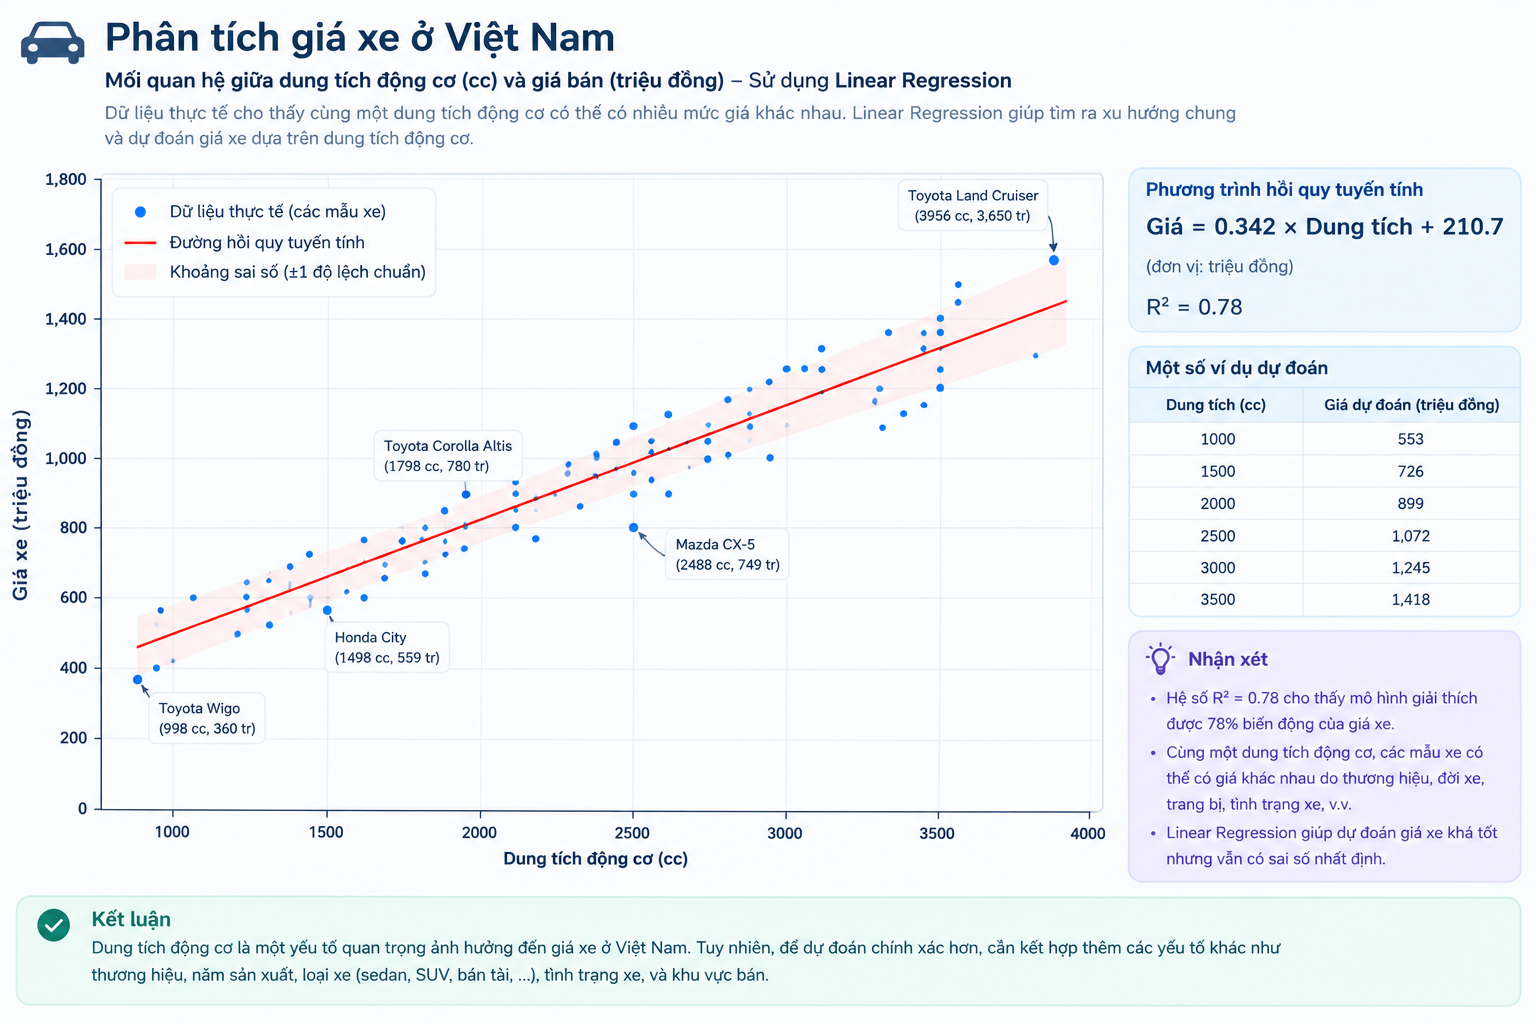
\includegraphics[width=0.9\textwidth]
    {../imgs/vietnam-car-price-regression.png}
    \caption{Minh họa phân tích giá xe theo năm sản xuất.}
    \label{fig:regression}
\end{figure}

Do chưa có kết quả đánh giá hồi quy trên tập test độc
lập được cung cấp trong phiên bản báo cáo này, chưa
đưa ra kết luận định lượng về khả năng dự đoán giá xe
trên các tin đăng mới. Các metric tính trên dữ liệu
huấn luyện chỉ phản ánh mức độ phù hợp của mô hình
với dữ liệu đã dùng để khớp.

\subsection{Trạng thái thực nghiệm của Vision Transformer}

Vision Transformer hiện mới ở giai đoạn đề xuất phương
pháp. Mô hình chưa được triển khai, huấn luyện hoặc
đánh giá trong dự án. Do đó, chưa có số liệu thực
nghiệm để báo cáo accuracy, loss, macro-F1 hoặc thời
gian huấn luyện của ViT.

Việc so sánh CNN với ViT chỉ có thể thực hiện sau khi
hoàn tất quá trình triển khai và đánh giá trên cùng
một tập test độc lập. Không thể kết luận ViT tốt hơn
hoặc kém hơn CNN dựa trên thiết kế phương pháp khi
chưa có kết quả thực nghiệm.

\section{Thảo luận và giới hạn}

\subsection{Giới hạn của Linear Regression}

Mô hình hồi quy minh họa sử dụng một biến đầu vào là
năm sản xuất. Do đó, mô hình không thể biểu diễn đầy
đủ ảnh hưởng của tình trạng xe, số kilomet đã đi,
xuất xứ, phiên bản và các yếu tố khác đến giá.

RMSE và $R^2$ của script hiện được tính trên dữ liệu
đã dùng để khớp mô hình. Ứng dụng Streamlit cũng hiển
thị mức độ phù hợp trên dữ liệu train. Vì chưa có tập
validation hoặc test độc lập, các metric này chưa phản
ánh đầy đủ khả năng dự đoán trên dữ liệu mới.

Ngoài ra, tên cột năm trong CSV được mô tả là
\texttt{Năm sản xuất}, trong khi script
\texttt{linear\_regression.py} được ghi nhận là truy
cập \texttt{Năm sản xuất:}. Sai khác này cần được
đồng bộ trước khi chạy lại script để tránh lỗi truy
cập cột.

Việc chuyển các cột văn bản sang số bằng cách trích
xuất số đầu tiên cũng là một giới hạn. Cách làm này
không bảo đảm giữ nguyên ý nghĩa của các thuộc tính
phân loại và có thể tạo ra đặc trưng không phù hợp
cho mô hình hồi quy.

\subsection{Giới hạn của CNN}

Kết quả accuracy 68,76\% và loss 1,1721 là kết quả
được lưu trong notebook, nhưng quy trình đánh giá
hiện tại chưa tách biệt hoàn toàn validation và test.
Việc sử dụng tập test trong quá trình huấn luyện có
thể ảnh hưởng đến tính độc lập của đánh giá cuối cùng.

Bên cạnh đó, augmentation ngẫu nhiên trong pipeline
đánh giá có thể khiến kết quả phụ thuộc vào phép biến
đổi được áp dụng. Cần kiểm tra phân bố số lượng ảnh
theo lớp, ảnh trùng lặp và những trường hợp dự đoán
sai để hiểu rõ hơn hiệu quả của mô hình.

\subsection{Giới hạn và kế hoạch đối với ViT}

ViT chưa được triển khai nên chưa thể đánh giá chi
phí tính toán, hiệu quả phân loại hoặc khả năng tổng
quát hóa trên bộ dữ liệu hiện có. Đây là giới hạn
về trạng thái triển khai, không phải bằng chứng cho
thấy phương pháp có hiệu quả thấp hoặc cao.

Hướng phát triển là fine-tune một mô hình ViT pretrained,
sau đó đánh giá trên cùng tập test với CNN. Việc so
sánh nên xem xét không chỉ accuracy mà còn macro-F1,
confusion matrix, thời gian huấn luyện và số lượng
tham số. Các kết quả chỉ được đưa vào báo cáo sau
khi thực nghiệm thực sự được hoàn thành.

\subsection{Khả năng tái lập}

Để tăng độ tin cậy, cần lưu lại phiên bản thư viện,
cấu hình mô hình, seed, cách chia dữ liệu và metric
của từng lần chạy. Với bài toán phân loại ảnh, cần
bảo đảm tập test không được sử dụng trong quá trình
lựa chọn mô hình. Với bài toán hồi quy, cần lưu lại
các bước tiền xử lý và đánh giá trên dữ liệu độc lập.

Các giao diện Streamlit và Gradio hỗ trợ minh họa
khả năng sử dụng của dự án, nhưng sự tồn tại của
giao diện không tự nó chứng minh hiệu năng dự đoán
hoặc khả năng tổng quát hóa của mô hình.

\section{Kết luận và hướng phát triển}

Dự án PPR501 Car Analysis kết hợp các kỹ thuật Machine
Learning và Deep Learning cho hai nhóm bài toán trong
lĩnh vực ô tô. Linear Regression được sử dụng để khảo
sát mối quan hệ giữa năm sản xuất và giá xe, trong khi
CNN được triển khai để phân loại hình ảnh thuộc bảy
nhóm xe. Streamlit cung cấp giao diện tương tác với
dữ liệu giá, còn Gradio hỗ trợ trình diễn khả năng
dự đoán ảnh.

Notebook CNN hiện ghi nhận accuracy khoảng 68,76\%
và loss khoảng 1,1721 sau 20 epoch. Tuy nhiên, do
quy trình đánh giá còn những hạn chế, kết quả cần
được xác minh lại trên tập test độc lập. Phần hồi
quy cũng cần bổ sung đánh giá trên dữ liệu chưa được
dùng để huấn luyện trước khi đưa ra kết luận về khả
năng dự đoán giá xe mới.

Vision Transformer được xác định là hướng mở rộng
cho bài toán phân loại ảnh xe. Vì mô hình chưa được
triển khai, báo cáo chưa đưa ra kết luận về hiệu năng
tương đối giữa ViT và CNN. Các bước tiếp theo gồm
chuẩn hóa dữ liệu, hoàn thiện quy trình đánh giá,
triển khai ViT pretrained và so sánh hai kiến trúc
trên cùng một tập test.

Những cải tiến này sẽ giúp dự án chuyển từ một hệ
thống minh họa các phương pháp Machine Learning
sang một quy trình thực nghiệm có thể tái lập và
có cơ sở đánh giá rõ ràng hơn.

\begin{credits}
    \subsubsection{\ackname}
    Nhóm xin cảm ơn giảng viên Nguyễn Xuân Sâm đã hướng
    dẫn nhóm trong học phần PPR501.

    \subsubsection{\discintname}
    Nhóm không có xung đột lợi ích cần công bố.
\end{credits}

\begin{thebibliography}{5}

    \bibitem{carprice}
    Kaggle: Automobile Dataset (Vietnam car prices).
    \url{https://www.kaggle.com/datasets/qucvinhdng/automobile-dataset}
    Truy cập ngày 18 tháng 10 năm 2026.

    \bibitem{carimages}
    Kshitij: Car Images Classification using CNN -- Dataset.
    Kaggle.
    \url{https://www.kaggle.com/code/kshitij192/car-images-classification-using-cnn/data}
    Truy cập ngày 18 tháng 10 năm 2026.

    \bibitem{repository}
    Nhóm PPR501: PPR501 Car Analysis.
    GitHub repository.
    \url{https://github.com/ptnghia3502/PPR501-car-analysis}
    Truy cập ngày 18 tháng 10 năm 2026.

    \bibitem{vit}
    Dosovitskiy, A., et al.:
    An Image is Worth 16x16 Words: Transformers for Image
    Recognition at Scale.
    In: International Conference on Learning Representations
    (ICLR) (2021).

    \bibitem{linearreg}
    Montgomery, D.C., Peck, E.A., Vining, G.G.:
    Introduction to Linear Regression Analysis.
    5th edn. Wiley (2012).

\end{thebibliography}

\end{document}
